%\documentclass[preprint,tightenlines,showpacs,showkeys,floatfix,
%nofootinbib,superscriptaddress,fleqn]{revtex4} 
\documentclass[floatfix,nofootinbib,superscriptaddress,fleqn,preprint]{revtex4} 
%\documentclass[aps,epsfig,tightlines,fleqn]{revtex4}
\usepackage[utf]{kotex}
\usepackage[HWP]{dhucs-interword}
\usepackage[dvips]{color}
\usepackage{graphicx}
\usepackage{bm}
%\usepackage{fancyhdr}
%\usepackage{dcolumn}
\usepackage{defcolor}
\usepackage{amsmath}
\usepackage{amsfonts}
\usepackage{amssymb}
\usepackage{amscd}
\usepackage{amsthm}
\usepackage[utf8]{inputenc}
 \usepackage{setspace}
 \usepackage{tikz}
%\pagestyle{fancy}

\begin{document}

\title{\Large 2022년 1학기 물리학 I: Quiz 7}
\author{김현철\footnote{Office: 5S-436D (면담시간 매주
    화요일-16:00$\sim$20:00)}} 
\email{hchkim@inha.ac.kr}
\affiliation{Hadron Theory Group, Department of Physics,
Inha University, Incheon 22212, Republic of Korea }
\date{Spring semester, 2022}


\vspace{1.cm}
\begin{abstract}
\noindent \textbf{ {\color{red}주의}: \color{blue} 단 한 번의 부정행위도 절대
  용납하지 않습니다. 적발 시, 학점은 F를 받게 됨은 물론이고,
  징계위원회에 회부합니다. One strike out임을 명심하세요.}\\
\\
문제는 다음 쪽부터 나옵니다.  \\ \\
{\bf Date:} 2022년 3월 23일 (수) 15:30-16:15 
\\
{\bf 학번:} \hspace{4cm}
{\bf 이름:} 

\end{abstract}
\maketitle

\noindent {\bf 문제 1 [10pt]}
탁구공의 질량은 2.3 g이고, 끝속력은 $9.0$ m/s이다. 탁구공이 자유낙하할
때 받는 끌림힘은 $bv^2$ 형태를 갖는다. 탁구공이 자유낙하를 할 때,
운동방정식을 세우고, $b$를 구하여라.  

\noindent {\bf 풀이}

자유낙하 하는 탁구공의 운동방정식은 다음과 같다.
\begin{align}
  \sum F = -bv^2+mg
\end{align}
시간이 충분히 지나 탁구공의 속력이 끝속력에 도달하면 탁구공의 속력은 
일정해진다. 이는 탁구공에 작용하는 합력이 0 임을 의미한다. 즉 끝속력을
$v_t$ 라고 하면,
\begin{align}
  bv_t^2 = mg,\,\,\, b =\frac{mg}{v_t^2}.
\end{align}
$m = 2.3\,\mathrm{g}$, $v_t = 9.0\,\mathrm{m/s}$ 이다. 따라서,
\begin{align}
  \begin{split}
    b &= \frac{(2.3\,\mathrm{g})(9.8\,\mathrm{m/s^2})}{( 9.0\,\mathrm{m/s})^2}  \\
    &= 0.28\,\mathrm{g/m}
  \end{split}
  \end{align}
  b 는 0.28 g/m 이다.
\vspace{1.cm}

\noindent {\bf 문제 2 [20pt]} 자동차가 급제동을 할 때, 바퀴가
잠겨서 미끄러지지 않도록 방지하는 장치를 잠김방지 브레이크
시스템(antilock braking system: ABS)이라고 부른다. 이 시스템에는
센서가 있어서 바퀴가 잠기는 것을 방지한다. 바퀴가 잠기려고 하면,
브레이크에 가해지는 힘을 줄이고, 다시 힘을 가하는 과정을 초당 15회
정도 반복한다. 그러면 자동차와 도로 사이의 마찰력을 최대로
유지한다. 이렇게 최대마찰력을 유지하는 브레이킹을 문턱
브레이킹(threshod braking)이라고 한다.
반면에 ABS가 없는 자동차의 경우에 급제동을 하면, 바퀴가
잠기게 된다. 이 경우에 제동거리도 길어지고, 운전자가 자동차의 주행
방향을 바로잡기가 힘들어진다.

어떤 자동차가 30 m/s의 속력으로 수평면을 주행하고 있다. 노면과 자동차
사이의 정지마찰계수와 운동마찰계수는 각각 $\mu_s=0.50$,
$\mu_k=0.40$이다. 
\begin{itemize}
\item[(가)] ABS가 있는 자동차가 문턱 브레이킹을 유지하면서 급제동을
  했을 때, 자동차의 제동거리는 얼마인가?
\item[(나)] ABS가 없는 자동차가 급제동을 했을 때 자동차의 제동거리는
  얼마인가?   
\end{itemize}
(자동차가 도로 위에서 미끄러지면(skidding), 타이어가 뜨거워지고,
마찰계수가 온도에 따라 바뀔 수 있다. 이 온도에 의한 효과는 여기서 무시하여라.)

\noindent {\bf 풀이}
\begin{itemize}
  \item[(가)] 문턱 브레이킹을 유지할 때 바퀴는 지면에 대해 계속 회전하므로 지면과 
  바퀴 사이에 정지 마찰력이 작용한다. 자동차의 질량을 $m$ 이라 하자. 운동 마찰력은,
  \begin{align}
    f_s = \mu_s N = \mu_s mg
  \end{align} 
이고 이 힘은 자동차가 정지할 때 까지 일정하게 작용한다. 즉,
\begin{align}
  ma = f_s,\,\,\, a = \frac{f_s}{m}=\mu_s g.
\end{align}
자동차의 가속도가 일정하므로 다음 공식을 적용할 수 있다.
\begin{align}
  2as = v^2_0-v^2.
\end{align}
자동차의 제동거리 $s$ 는 다음과 같다.
\begin{align}
  \begin{split}\label{eq:2-1}
    s &= \frac{v^2_0-v^2}{2a} = \frac{v^2_0-v^2}{2\mu_s g}  \\
    &= \frac{(30\,\mathrm{m/s})^2}{2(0.50)(9.8\,\mathrm{m/s^2})}  \\
    &= 92\,\mathrm{m}
  \end{split}
\end{align}
ABS가 작동한다면 이 자동차의 제동거리는 92 m 이다.
  \item[(나)] ABS 가 작동하지 않는다면 제동하는 동안 바퀴가 회전하지 않으므로 
  지면에 대해 운동 마찰력이 작용한다. 식 (\ref{eq:2-1}) 에 의해 이 경우의 
  제동거리 $s$ 는,
  \begin{align}
    \begin{split}
      s &= \frac{v^2_0-v^2}{2a} = \frac{v^2_0-v^2}{2\mu_k g}  \\
      &= \frac{(30\,\mathrm{m/s})^2}{2(0.40)(9.8\,\mathrm{m/s^2})}  \\
      &= 110\,\mathrm{m}
    \end{split}
  \end{align}
  ABS가 작동하지 않는다면 이 자동차의 제동거리는 110 m 이다.
\end{itemize}

\vspace{1.cm}

\noindent {\bf 문제 3 [20pt]}
그림~\ref{fig:3}에서처럼 세 힘을 어떤 물체에 가해 쓸림이 없는
수평면에서 3.00 m를 이동시켰다. 이 세 힘의 크기는 각각
$F_1=5.00$ N, $F_2=9.00$ N, $F_3=3.00$ N이고, $\vec{F}_2$와 수평선 
사이의 각은 $\theta=60.0^\circ$이다. 이 물체가 이동하는 동안, 
\begin{figure}[ht]
  \centering
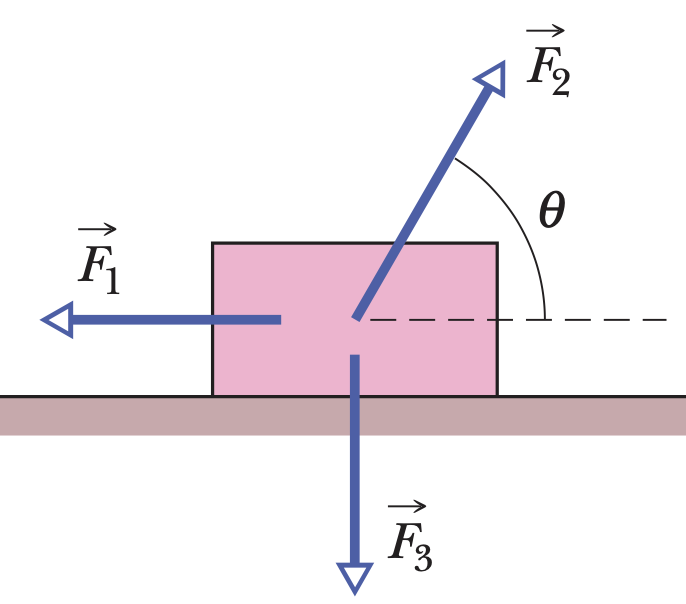
\includegraphics[scale=0.45]{Qfig7-3-20220323.png}  
  \caption{문제 3}
  \label{fig:3}
\end{figure}
\begin{itemize}
\item[(가)] 세 힘이 물체에 해준 알짜일은 얼마인가?
\item[(나)] 이 물체의 운동에너지는 증가하였는가, 감소하였는가?
\end{itemize}


\begin{figure}
  \begin{tikzpicture}
    \draw (-3,0) -- (3,0) node [above] {$+x$};
    \draw [red,very thick,-latex] (0.1,0) -- (1,0) 
    node [above,black] {$|\vec{F_2}|\cos{\theta}$};
    \draw [red,very thick,-latex] (-0.1,0) -- (-1.6,0) 
    node [above,black] {$|\vec{F_1}|$};
    \draw (0,-2.5) -- (0,2.5) node [right] {$+y$};
    \draw [blue,very thick,-latex] (0,0.1) -- (0,1.5) 
    node [right,black] {$|\vec{F_2}|\sin{\theta}$};
    \draw [blue,very thick,-latex] (0,-0.1) -- (0,-1) 
    node [right,black] {$|\vec{F_3}|$};
  \end{tikzpicture} \caption{Free body diagram}
\end{figure}


\noindent {\bf 풀이}
\begin{itemize}
  \item [(가)] 물체의 오른쪽을 $+x$ 방향, 위쪽을 $+y$ 방향이라 하자.
   물체에 $x$ 방향으로 작용하는 합력은 다음과 같다.
   \begin{align}
     F_x =|\vec{F_2}|\cos{\theta}-|\vec{F_1}|
   \end{align}
   물체에 $y$ 방향으로 작용하는 합력은 다음과 같다.
   \begin{align}
      F_y =|\vec{F_2}|\sin{\theta}-|\vec{F_3}|
   \end{align}
   이 물체는 합력이 작용하는 방향으로 움직인다. 따라서 운동 방향과 합력이 이루는 각도는 
   $0^\circ$ 이다. 따라서, 
   \begin{align}
    \begin{split}
      W &= \vec{F}\cdot\vec{d}=\left|\vec{F}\right||\vec{d}|
      =\sqrt{{F_x}^2+{F_y}^2}|\vec{d}|  \\
      &=\sqrt{\left(|\vec{F_2}|\cos{\theta}
      -|\vec{F_1}|\right)^2+\left(|\vec{F_2}|\sin{\theta}
      -|\vec{F_3}|\right)^2}|\vec{d}|.
    \end{split}
  \end{align}
  이 때 세 힘이 해준 알짜일은 다음과 같다.
  \begin{align}
    \begin{split}
      W&=\sqrt{\left(|\vec{F_2}|\cos{\theta}
      -|\vec{F_1}|\right)^2+\left(|\vec{F_2}|\sin{\theta}
      -|\vec{F_3}|\right)^2}|\vec{d}| \\
      &= \left( \sqrt{\left(9.00\times\frac{1}{2}
      -5.00\right)^2+\left(9.00\times\frac{\sqrt{3}}{2}
      -3.00\right)^2 }\right)(3.00)\,\mathrm{J} \\
      &=14.5\,\mathrm{J}
    \end{split}
    \end{align}
    세 힘은 물체에게 $14.5\,\mathrm{J}$ 만큼의 일을 해주었다.
%---------------------------------------------------
  %  따라서 물체에 작용하는 합력은 다음과 같다.
  %  \begin{align}
  %    \begin{split}
  %      \sum\vec{F} &= \left(|\vec{F_2}|\cos{\theta}
  %      -|\vec{F_1}|\right)\hat{\bm{i}}
  %      + \left(|\vec{F_2}|\sin{\theta}
  %      -|\vec{F_3}|\right)\hat{\bm{j}}  \\
  %     &=\left((9.00\,\mathrm{N})\cos{60.0^\circ}
  %     -(5.00\,\mathrm{N})\right)\hat{\bm{i}}
  %      + \left((9.00\,\mathrm{N})\sin{60.0^\circ}
  %      -(3.00\,\mathrm{N})\right)\hat{\bm{j}} \\
  %      &=\left(-0.50\,\hat{\bm{i}}
  %       + \left( 4.50\sqrt{3}
  %       -3.00\right)\hat{\bm{j}}\right)\,\mathrm{N}
  %    \end{split}
  %  \end{align}
  ------------- y 방향 힘이 0 인 경우 ----------
 물체는 수평면에서 이동하였으므로 $x$ 방향으로 가해진 힘 만이 물체에 일을 해주었다. 
 따라서 물체가 움직인 거리를 $d$ 라 하면 세 힘이 물체에 해준 알짜일은 다음과 같다.
 \begin{align}
  \begin{split}
    W &= \sum F_x\,d= \left(|\vec{F_1}|-|\vec{F_2}|\cos{\theta}\right)\,d \\
    &= \left((5.00\,\mathrm{N})-(9.00\,\mathrm{N})\cos{60.0^\circ}\right)
    (3.00\,\mathrm{m})  \\
    &= 1.50\,\mathrm{J}
  \end{split}
 \end{align}
  \item [(나)] 외부에서 물체에 일을 해주었으므로 이 물체의 운동에너지는 
  증가하였다.
\end{itemize}

\vspace{1.cm}

\noindent {\bf 문제 4 [10pt]} 
수평 바닥에 $37.0^\circ$의 각도로 122 N의 힘이 100 kg의 토막에
작용하여 토막이 5.00 m/s의 일정한 속력으로 수평바닥을 따라 끌려가고
있다. 힘이 토막에 한 일의 시간변화율은 얼마인가?  \\

\begin{figure}
  \begin{tikzpicture}
    \draw (-3,0) -- (3,0) node [right] {$+x$};
    \draw [red,very thick,-latex] (0.1,0) -- (2,0) 
    node [above,black] {$F\cos{\theta}$};
    \draw [red,very thick,-latex] (-0.1,0) -- (-2,0) 
    node [above,black] {$f_k$};
    \draw (0,-2.5) -- (0,2.5) node [right] {$+y$};
    \draw [blue,very thick,-latex] (0.07,0.1) -- (0.07,1.3) 
    node [right,black] {$F\sin{\theta}$};
    \draw [blue,very thick,-latex] (-0.07,0.1) -- (-0.07,0.9) 
    node [left,black] {$N$};
    \draw [blue,very thick,-latex] (0,-0.1) -- (0,-2.2) 
    node [right,black] {$mg$};
  \end{tikzpicture} \caption{Free body diagram}
\end{figure}

\noindent {\bf 풀이} 물체의 오른쪽을 $+x$ 방향, 위쪽을 $+y$ 방향이라 하자.
토막이 일정한 속력으로 수평바닥을 따라 끌려가고 있으므로 토막에 작용하는 합력의 
$x$ 방향 성분은 0 이어야 한다. 따라서,
\begin{align}
  F_x = F\cos{\theta}-f_k = F\cos{\theta}-\mu_k N=0.
\end{align}
토막이 $y$ 방향으로 가속 운동하지 않으므로 합력의 $y$ 방향 성분 또한 0 이어야 한다. 
토막이 바닥으로 부터 받는 수직 항력을 $N$ 이라 하면,
\begin{align}
  F_y = F\sin{\theta}-mg+N = 0,\,\,\,N = mg-F\sin{\theta}
\end{align}
힘이 토막에 한 일을 계산해보자. 토막은 $x$ 방향으로 움직이므로,
\begin{align}
  W = \vec{F}\cdot\vec{d} = F_x d = F\cos
\end{align}

%------------------
% 토막이 일정한 속력으로 수평바닥을 끌려가고 있으므로 힘의 
% 수평 성분만이 토막에 일을 해주었다. 힘이 토막에 한 일은 다음과 같다.
% \begin{align}
%   W = F\,d = F_x\,d = (F\cos{\theta})d
% \end{align}
% 이 토막은 등속도로 운동하므로,
% \begin{align}
%   d=vt,\,\,\,W=(F\cos{\theta})vt
% \end{align}
% 이 일의 시간변화율은 이 일을 시간에 대해 미분한 값이다.
% \begin{align}
%   \begin{split}
%     \frac{dW}{dt} &= (F\cos{\theta})v  \\
%     &= (122\,\mathrm{N})(\cos{37.0^\circ})(5.00\,\mathrm{m/s})  \\
%     &= 467\,\mathrm{W}
%   \end{split}
% \end{align}
% 힘이 토막에 한 일의 시간변화율은 467 W 이다.


\end{document}